\begin{frame}
    \frametitle{Data Pengukuran Kamera}

    Data yang ditangkap kamera berupa matriks tiga dimensi berukuran
    \begin{equation}
        w \times h \times 3
    \end{equation}
    $w$ merupakan tinggi gambar, $h$ merupakan lebar gambar, dan 3 menyatakan intensitas warna piksel dalam bentuk vektor warna merah, hijau, dan biru.

    Kamera mengambil gambar setiap $\frac{1}{30}$ detik dan akan disimpan ke dalam memori \textit{buffer} dalam bentuk set
    \begin{equation}
        \lbrace \mathbf{R}^{w \times h \times 3}, timestamp \rbrace
    \end{equation}
    Agar error yang disebabkan oleh perbedaan waktu kecil, algoritma yang diusulkan akan memilih set yang memiliki timestamp terdekat ke timestamp data Lidar.
\end{frame}


\begin{frame}
    \frametitle{Data Pengukuran Lidar}

    Lidar menghasilkan titik-titik jarak dari Lidar ke objek yang disebut dengan \textit{point cloud}.

    Point Cloud ($\mathbf{P}$) merupakan kumpulan dari set posisi titik di ruang tiga dimensi

    \begin{equation}
        \mathbf{P} = \lbrace x, y, z \rbrace
    \end{equation}

    $x, y,$ dan $z$ merupakan jarak eucledian. Data point cloud yang dihasilkan oleh Lidar sudah memiliki timestamp. Timestamp ini akan digunakan untuk melakukan sinkronisasi waktu antara Lidar dan Kamera.
\end{frame}


\begin{frame}[allowframebreaks]
    \frametitle{Data Pengukuran GPS. Bagian}

    Data yang diterima oleh sensor GPS berbentuk data teks (ASCII) dengan format standar National Marine Electronics Association (NMEA).

    \textbf{\$GPGGA, 181908.00, 3404.7041778, N, 0744.3966270, W, 4, 13, 1.00, 495.144, M, 29.200, M, 0.10,0000 *40}

    \begin{itemize}
        \item \textbf{GP} menyatakan bahwa data ini merupakan data dari GPS. GLONASS menggunakan \textbf{GL}, dan Beidou menggunakan \textbf{BD}.
        \item \textbf{181908.00} merupakan timestamp UTC dengan format: HHMMSS.mm
        \item \textbf{3404.7041778} merupakan latitude. format : DDMM.MMMMMMM
        \item \textbf{N} menunjukkan latitude Utara
        \item \textbf{0744.3966270} merupakan longitude. format : DDMM.MMMMMMM
        \item \textbf{W} menunjukkan longitude Barat
        \item \textbf{4} menunjukkan kualitas pengukuran (4 = presisi hingga cm)
        \item \textbf{13} menunjukkan jumlah satelit yang digunakan
        \item \textbf{*40} menunjukkan checksum data
    \end{itemize}
\end{frame}


\begin{frame}
    \frametitle{Data Pengukuran INS}

    INS merupakan sensor yang terdiri dari Akselerometer dan Giroskop. Akselerometer mengukur gaya spesifik ($sf$) yang bekerja pada tiap sumbu, sementara Giroskop mengukur kecepatan angular ($p, q, r$) terhadap ketiga sumbu tersebut \cite{alam2016ins}.
\end{frame}


\begin{frame}[allowframebreaks]
    \frametitle{Eucledian Clustering. Bagian}

    Sebelum dapat digabungkan, data yang dihasilkan oleh Lidar perlu diproses terlebih dahulu. Centroid dari cluster 3D point cloud pembacaan Lidar dicari menggunakan Eucledian Clustering Algorithm \cite{schutze2008introduction}.

    Algoritma Eucledian Clustering mengelompokkan point cloud deteksi Lidar berdasarkan kedekatannya dengan point cloud di sekitarnya.

    \begin{equation}
        P = (p_1, p_2, \cdots, p_n) \text{ dimana } P \in R^{3 \times n}
    \end{equation}
    \begin{equation}
        K = (\mu_1, \mu_2, \cdots, \mu_m) \text{ dimana } K \in R^{3 \times m}
    \end{equation}

    $P$ merupakan kumpulan dari point cloud $p$ Lidar, $K$ merupakan kumpulan dari cluster $k$ dengan titik centroid cluster yang posisinya belum diketahui $\mu$.

    \pagebreak

    Eucedian Clustering mengelompokkan point terdekat dari centroid suatu cluster ke dalam cluster tersebut. Posisi centroid dari tiap cluster dapat berubah bergantung posisi dari kumpulan point yang ada dalam cluster.

    Untuk mengetahui sebaik apa suatu cluster, perlu dicari jumlahan jarak terkecil dari tiap titik di suatu cluster ke centroid dari cluster tersebut \cite{schutze2008introduction} yang dapat dituliskan sebagai fungsi objektif $\mathcal{L}$

    \begin{equation}
        \mathcal{L} = \sum_{j=1}^{m}\sum_{i=1}^{n}\left\|p_{i}-\mu_{j}\right\|^{2}
        \label{eq: objective-cluster}
    \end{equation}

    \pagebreak

    Algoritma Eucledian Clustering mencoba meminimalkan $\mathcal{L}$ melalui tahapan iteratif:
        \begin{enumerate}
            \item inisialisasi $\mu_1, \cdots, \mu_m$ dengan memilih point acak
            \item memilih poin optimal untuk titik centroid $\mu$ tetap
            \item memilih centroid optimal berdasarkan poin di dalam cluster
            \item ulangi langkah 2-3 hingga hasil konvergen
        \end{enumerate}
\end{frame}


\begin{frame}[allowframebreaks]
    \frametitle{Persamaan Mekanisasi INS. Bagian}
    
    Persamaan mekanisasi diperlukan oleh INS untuk merepresentasikan hasil pengukuran dari INS yang berupa kecepatan angular $p, q, r$ dan gaya spesifik $sf$ menjadi Posisi, Kecepatan, dan Attitude (PVA).

    Seperti pada \cite{nemra2010robust}, perubahan attitude kendaraan $\dot{\theta}, \dot{\phi}, \dot{\psi}$ dapat dicari dari kecepatan angular dan bias giroskop $b_g$ yang telah kita ketahui menggunakan persamaan (\ref{eq: ins-attitude-change})

    \begin{equation}
        \begin{array}{c}
        {\left[\begin{array}{l}
        \dot{\theta} \\
        \dot{\theta} \\
        \dot{\psi}
        \end{array}\right]=\left[\begin{array}{ccc}
        1 & \sin (\phi) \tan (\theta) & \cos (\phi) \tan (\theta) \\
        0 & \cos (\phi) & -\sin (\phi) \\
        0 & \sin (\phi) \sec (\theta) & \cos (\phi) \sec (\theta)
        \end{array}\right]}
        \cdot\left(\left[\begin{array}{l}
        p \\
        q \\
        r
        \end{array}\right]-\left[\begin{array}{c}
        b_{g x} \\
        b_{g y} \\
        b_{g z}
        \end{array}\right]\right)
        \end{array}
        \label{eq: ins-attitude-change}
    \end{equation}

    \pagebreak

    perubahan kecepatan $\dot{u}, \dot{v}, \dot{w}$ dapat dicari menggunakan persamaan (\ref{eq: ins-speed-change}) dimana bias akselerometer $b_a$ juga diperhatikan.

    \begin{equation}
        \left[\begin{array}{c}
        \dot{u} \\
        \dot{v} \\
        \dot{w}
        \end{array}\right]=C_{b n}{ }^{T}\left[\begin{array}{l}
        0 \\
        0 \\
        g
        \end{array}\right]+\left(\left[\begin{array}{l}
        s f_{x} \\
        s f_{y} \\
        s f_{z}
        \end{array}\right]-\left[\begin{array}{l}
        b_{a x} \\
        b_{a y} \\
        b_{a z}
        \end{array}\right]\right)+\left[\begin{array}{c}
        v r-w q \\
        -u r+w p \\
        u q-v p
        \end{array}\right]
        \label{eq: ins-speed-change}
    \end{equation}

    $C_{b n}$ adalah Direct Cosine Transform Matrix yang mengubah vektor dari frame body ke frame North East Down (NED) \cite{alam2016ins} yang dapat dituliskan sebagai (\ref{eq: ins-cbn}).

    \begin{equation}
        \begin{array}{l}
        C_{b n}
        =\left[\begin{array}{ccc}
        \cos \phi \cos \theta & \sin \theta \sin \psi \cos \phi-\sin \phi \cos \psi & \sin \psi \sin \phi+\cos \phi \cos \psi \sin \theta \\
        \cos \theta \sin \phi & \cos \psi \cos \phi+\sin \phi \sin \psi \sin \theta & \sin \theta \sin \psi \sin \phi-\cos \phi \sin \psi \\
        -\sin \theta & \cos \psi \sin \theta & \cos \psi \cos \theta
        \end{array}\right]
        \end{array}
        \label{eq: ins-cbn}
    \end{equation}

    \pagebreak

    Kecepatan perlu diubah dari frame body ke frame NED dan dapat dituliskan sebagai (\ref{eq: ins-speed}), sementara bias gyro dan akselerometer merupakan nilai konstan (\ref{eq: ins-constant-bias}).

    \begin{equation}
        \left[\begin{array}{l}
        \dot{X} \\
        \dot{Y} \\
        \dot{Z}
        \end{array}\right]=C_{b n}\left[\begin{array}{l}
        u \\
        v \\
        z
        \end{array}\right]
        \label{eq: ins-speed}
    \end{equation}
    \begin{equation}
        \left[\begin{array}{c}
        \dot{b_{g x}}\\
        \dot{b_{g y}}\\
        \dot{b_{g z}}
        \end{array}\right]=\left[\begin{array}{l}
        \dot{b_{a x}} \\
        \dot{b_{a y}} \\
        \dot{b_{a z}}
        \end{array}\right]=\left[\begin{array}{l}
            0 \\
            0 \\
            0
        \end{array}\right]
        \label{eq: ins-constant-bias}
    \end{equation}

    \begin{center}
        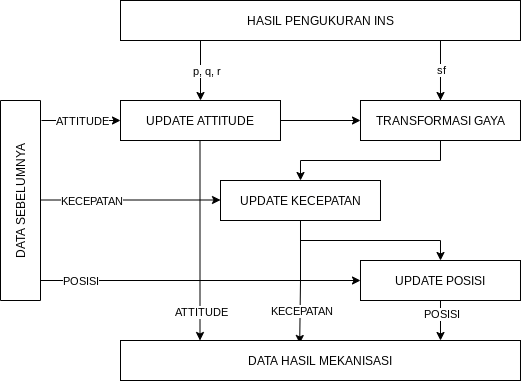
\includegraphics[width=.6\textwidth]{3-INS-mechanization-v3.png}
    \end{center}
\end{frame}


\begin{frame}
    \frametitle{Struktur Data Lidar Setelah Proses Eucledian Clustering}

    Hasil Algoritma Eucledian Clustering pada deteksi Lidar berupa titik koordinat tiga dimensi dengan data berbentuk nilai centroid.
    \begin{equation}
        w_{\text{lidar},i}^{t}=\left\{x_{\text{lidar}, i}^{t}, y_{\text{lidar}, i}^{t}, z_{\text{lidar},i}^{t}\right\}
    \end{equation}
    Karena kendaraan bergerak pada bidang datar, maka posisi terhadap sumbu $z$ dapat diabaikan \cite{kim2020EKFradarlidar}, sehingga:
    \begin{equation}
        w_{\text{lidar},i}^{t}=\left\{x_{\text{lidar}, i}^{t}, y_{\text{lidar}, i}^{t}\right\}
    \end{equation}
    Kecepatan dari halangan tidak didapatkan dari pengukuran secara langsung sehingga perlu diestimasi berdasarkan perubahan posisi halangan terhadap waktu.
\end{frame}


\begin{frame}
    \frametitle{Struktur Data Kamera Setelah Proses 3D RPN}

    Hasil deteksi 3D RPN yang dilakukan pada kamera berupa titik koordinat tiga dimensi dari centroid, dan klasifikasi jenis objek yang terdeteksi.
    \begin{equation}
        w_{\text{kamera},i}^{t}=\left\{x_{\text{kamera}, i}^{t}, y_{\text{kamera}, i}^{t}, z_{\text{kamera},i}^{t}, \alpha_{\text{kamera},i}^{t}\right\}
    \end{equation}
    Karena halangan bergerak pada bidang datar, maka posisi terhadap sumbu $z$ dapat diabaikan \cite{kim2020EKFradarlidar}, sehingga:
    \begin{equation}
        w_{\text{kamera},i}^{t}=\left\{x_{\text{kamera}, i}^{t}, y_{\text{kamera}, i}^{t}, \alpha_{\text{kamera},i}^{t}\right\}
    \end{equation}
\end{frame}


\begin{frame}[allowframebreaks]
    \frametitle{Model Filter Gabungan Lidar dan Kamera. Bagian}

    Setiap track perlu memiliki data posisi, kecepatan, dan heading. Karena itu, state ($\varphi$) yang disimpan dalam setiap track mencakup posisi ($x_{i}^{t}, y_{i}^{t}$), kecepatan ($V_{i}^{t}$), dan arah heading dari halangan ($\alpha_{i}^{t}$) relatif terhadap mobil otonom. Pitch dan roll dari halangan dapat diabaikan karena mobil berjalan pada bidang datar.

    \begin{equation}
        \varphi_{i}^{t}=\left\{x_{i}^{t}, y_{i}^{t}, V_{i}^{t}, \alpha_{i}^{t}\right\}
    \end{equation}

    Vektor pengukuran gabungan dari Kalman Filter ini merupakan gabungan dari pengukuran posisi oleh lidar dan kamera.
    
    \begin{equation}
        z_{i}^{t}=\left\{x_{\text {lidar}, i}^{t}, y_{\text {lidar }, i}^{t}, x_{\text {kamera}, i}^{t} y_{\text {kamera}, i}^{t}, \alpha_{i}^{t}\right\}
        \label{eq: 3-meas-vec}
    \end{equation}

    Estimasi posisi halangan bisa didapatkan berdasarkan kinematika gerak linier

    \begin{equation}
        x_{i}^{t} = x_{i}^{t-1} + \Delta t \cdot V_{i}^{t-1} \cos \left(\alpha_{i}^{t-1}\right)
    \end{equation}
    \begin{equation}
        y_{i}^{t} = y_{i}^{t-1} + \Delta t \cdot V_{i}^{t-1} \sin \left(\alpha_{i}^{t-1}\right)
    \end{equation}

    Sehingga model proses $f$ dapat dituliskan sebagai
    \begin{equation}
        f_{i}^{t-1}=\left[\begin{array}{c}
        x_{i}^{t-1}+\Delta t V_{i}^{t-1} \cos \left(\alpha_{i}^{t-1}\right) \\
        x_{i}^{t-1}+\Delta t V_{i}^{t-1} \sin \left(\alpha_{i}^{t-1}\right) \\
        V_{i}^{t-1} \\
        \alpha_{i}^{t-1}
        \end{array}\right]
        \label{eq:model-process}
    \end{equation}

    Persamaan (\ref{eq:model-process}) merupakan persamaan nonlinier, sehingga perlu dilinerisasi menggunakan operasi jacobi pada $f$
    \begin{equation}
        F_{i}^{t-1}=\left[\begin{array}{cccc}
        1 & 0 & \Delta t \cos \left(\alpha_{i}^{t-1}\right) & 0 \\
        0 & 1 & \Delta t \sin \left(\alpha_{i}^{t-1}\right) & 0 \\
        0 & 0 & 1 & 0 \\
        0 & 0 & 0 & 1
        \end{array}\right]
    \end{equation}

    Vektor pengukuran dapat dituliskan sebagai
    \begin{equation}
        z_{i}^{t}=\left[\begin{array}{c}
        x_{\text {lidar }, i}^{t} \\
        y_{\text {lidar }, i}^{t} \\
        x_{\text {kamera }, i}^{t} \\
        y_{\text {kamera }, i}^{t} \\
        \alpha_{\text {kamera , } i}^{t}
        \end{array}\right]^{T}=\left[\begin{array}{c}
        x_{i}^{t-1}+\Delta \mathrm{t} V_{i}^{t-1} \cos \left(\alpha_{i}^{t-1}\right) \\
        y_{i}^{t-1}+\Delta \mathrm{t} V_{i}^{t-1} \sin \left(\alpha_{i}^{t-1}\right) \\
        x_{i}^{t-1}+\Delta \mathrm{t} V_{i}^{t-1} \cos \left(\alpha_{i}^{t-1}\right) \\
        y_{i}^{t-1}+\Delta \mathrm{t} V_{i}^{t-1} \sin \left(\alpha_{i}^{t-1}\right) \\
        \alpha_{i}^{t-1}
        \end{array}\right]^T
    \end{equation}

    Matriks model pengukuran $H$ dapat dicari dengan melakukan operasi jacobi pada z

    \begin{equation}
        H_{i}^{t}=\left[\begin{array}{ccccc}
        1 & 0 & \Delta \mathrm{t} \cos \left(\alpha_{i}^{t-1}\right) & 0 \\
        0 & 1 & \Delta \mathrm{t} \sin \left(\alpha_{i}^{t-1}\right) & 0 \\
        1 & 0 & \Delta \mathrm{t} \cos \left(\alpha_{i}^{t-1}\right) & 0 \\
        0 & 1 & \Delta \mathrm{t} \sin \left(\alpha_{i}^{t-1}\right) & 0 \\
        0 & 0 & 0 & 1 \\
        \end{array}\right]
    \end{equation}
\end{frame}


\begin{frame}
    \frametitle{Proses Update Gabungan Lidar dan Kamera}

    Vektor state $\varphi_{i}^{t}$ diestimasi dengan matriks $F_{i}^{t-1}$ menggunakan (\ref{eq: lidar-cam-state-est}). Selanjutnya kovarian error $P_{i}^{t}$ dicari dengan (\ref{eq: lidar-cam-err-cov}) dimana $Q$ merupakan noise sistem.
        \begin{equation}
            \varphi_{\bar{i}}^{-}=\mathrm{F}_{i}^{t-1} \varphi_{i}^{t-1}
            \label{eq: lidar-cam-state-est}
        \end{equation}
        \begin{equation}
            P_{i}^{t}=\mathrm{F}_{i}^{t-1} P_{i}^{t-1} \mathrm{~F}_{i}^{t-1^{T}}+Q
            \label{eq: lidar-cam-err-cov}
        \end{equation}
        \begin{equation}
            K_{i}^{t}=P_{i}^{t} H_{i}^{t-1^{T}}\left[H_{i}^{t-1} P_{i}^{t} H_{i}^{t-1^{T}}+R_{i}\right]^{-1}
            \label{eq: lidar-cam-kalman-gain}
        \end{equation}
        \begin{equation}
            \varphi_{i}^{t}=\varphi_{i}^{t-1}+K_{i}^{t}\left[z_{i}^{t}-H_{i}^{t-1} \varphi_{i}^{t}\right]
            \label{eq: lidar-cam-state}
        \end{equation}
        Gain Kalman didapat dari (\ref{eq: lidar-cam-kalman-gain}) dimana $R_j$ merupakan noise pengukuran. Kalman gain $K$, hasil pengukuran, dan prediksi kemudian digunakan untuk mencari $\varphi_{j}^{t}$ menggunakan (\ref{eq: lidar-cam-state}). Update dari error kovarian didapat dari $K$ yang telah di update.
        \begin{equation}
            P_{i}^{t}=\left[I-K_{i}^{t} H_{i}^{t}\right] P_{i}^{t-1}
        \end{equation}
\end{frame}


\begin{frame}
    \frametitle{Struktur Data INS}

    Data INS berupa gaya spesifik ($sf$) dan kecepatan angular ($p, q, r$) dapat diproses dan ditransformasi untuk mendapatkan posisi, kecepatan dan attitude dari mobil otonom.
    \begin{equation}
        u=\left[s f_{x}, s f_{y}, s f_{z}, p, q, r\right]^{T}
        \label{eq: ins-measure}
    \end{equation}
    Data pengukuran yang didapatkan dari INS direpresentasikan dengan (\ref{eq: ins-measure}) dimana $p, q, r$ merupakan kecepatan angular  
\end{frame}


\begin{frame}
    \frametitle{Struktur Data GPS}

    GPS merupakan sensor navigasi berbasis satelit yang dapat digunakan untuk menentukan posisi.
    \begin{equation}
        y=[X, Y, Z]^{T}
        \label{eq: gps-ins-measurement-vector}
    \end{equation}
    Data pengukuran yang didapatkan dari GPS direpresentasikan dengan (\ref{eq: gps-ins-measurement-vector}) dimana $X, Y, Z$ merupakan posisi.
\end{frame}


\begin{frame}[allowframebreaks]
    \frametitle{Model Filter Gabungan INS dan GPS. Bagian}

    Model yang digunakan pada EKF dari fusi INS dan GPS didefinisikan sebagai sistem nonlinier (\ref{eq: ins-gps-nonlin}) dengan vektor state (\ref{eq: ins-gps-state})
    \begin{equation}
        \left\{\begin{array}{l}
        \dot{x}(t)=f(x(t), u(t), t) \\
        y(t)=h(x(t), g(t), t)
        \end{array}\right.
        \label{eq: ins-gps-nonlin}
    \end{equation}
    \begin{equation}
        x=\left[X, Y, Z, u, v, w, \theta, \phi, \psi, b_{g x}, b_{g y}, b_{g z}, b_{a x}, b_{a y}, b_{a z}\right]^{T}
        \label{eq: ins-gps-state}
    \end{equation}
    $u, v, w$ merupakan kecepatan; $\theta, \phi, \psi$ merupakan attitude; $b_{g}$ merupakan bias gyro; dan $b_{a}$ merupakan bias akselerometer.

    \pagebreak

    Persamaan (\ref{eq: ins-attitude-change}; \ref{eq: ins-speed-change}; \ref{eq: ins-cbn}; \ref{eq: ins-speed}; \ref{eq: ins-constant-bias}) dapat disubstitusikan ke persamaan (\ref{eq: ins-gps-nonlin}) untuk mendapatkan model state $f(x,u,t)$
    \begin{equation}
        \footnotesize
        f(x, u, t) = \left\{\begin{array}{l}
            C_{b n}\left[\begin{array}{l}
                u \\
                v \\
                z
            \end{array}\right] \\
            C_{b n}{ }^{T}\left[\begin{array}{l}
                0 \\
                0 \\
                g
                \end{array}\right]+\left(\left[\begin{array}{l}
                s f_{x} \\
                s f_{y} \\
                s f_{z}
                \end{array}\right]-\left[\begin{array}{l}
                b_{a x} \\
                b_{a y} \\
                b_{a z}
                \end{array}\right]\right)+\left[\begin{array}{c}
                v r-w q \\
                -u r+w p \\
                u q-v p
            \end{array}\right] \\
            \left[\begin{array}{ccc}
                1 & \sin (\phi) \tan (\theta) & \cos (\phi) \tan (\theta) \\
                0 & \cos (\phi) & -\sin (\phi) \\
                0 & \sin (\phi) \sec (\theta) & \cos (\phi) \sec (\theta)
                \end{array}\right]
                \left(\left[\begin{array}{l}
                p \\
                q \\
                r
                \end{array}\right]-\left[\begin{array}{c}
                b_{g x} \\
                b_{g y} \\
                b_{g z}
            \end{array}\right]\right) \\
            \left[\begin{array}{l}
                0 \\
                0 \\
                0
            \end{array}\right] \\
            \left[\begin{array}{l}
                0 \\
                0 \\
                0
            \end{array}\right]
        \end{array}\right.
        \label{eq: ins-model-state-eqn}
    \end{equation}

    \pagebreak

    Model observasi $H$ terpengaruh oleh $C_{b n}$ karena kecepatan pada state dan measurement berada pada frame yang berbeda
    \begin{equation}
        \begin{array}{l}
        h(x, g, t)
        =\left[\begin{array}{lll}
        I_{3x3} & 0_{3x3} & 0_{9x3} \\
        0_{3x3} & C_{b n}^T & 0_{9x3}
        \end{array}\right]
        \end{array}
        \label{eq: ins-model-observation}
    \end{equation}
    Sistem dituliskan sebagai model nonlinear waktu diskrit (\ref{eq: ins-gps-state-discrete}), dengan nilai $f$ dan $h$ yang sudah didefinisikan di (\ref{eq: ins-model-state-eqn}) dan (\ref{eq: ins-model-observation}) \cite{alam2016ins}.
    \begin{equation}
        \left\{\begin{array}{c}
        x_{k}=f\left(x_{k-1}, u_{k-1}, w_{k-1}\right) \\
        y_{k}=h\left(x_{k}, v_{k}\right)
        \end{array}\right.
        \label{eq: ins-gps-state-discrete}
    \end{equation}
    $x_k$ merupakan state pada waktu $k$; $w_k$ noise sistem pada waktu $k$; $y_k$ pengukuran pada waktu $k$; dan $v_k$ noise pengukuran pada waktu $k$.

    \pagebreak

    \begin{equation}
        F_{k-1}=\left.\frac{\partial f_{k-1}}{\partial x}\right|_{\hat{x}_{k-1}^{+}}
        \label{eq: ins-gps-jacobi-state-component}
    \end{equation}
    \begin{equation}
        L_{k-1}=\left.\frac{\partial f_{k-1}}{\partial w}\right|_{\hat{x}_{k-1}^{+}}
        \label{eq: ins-gps-jacobi-state-noise}
    \end{equation}
    \begin{equation}
        \bar{u}_{k-1}=f_{k-1}\left(\hat{x}_{k-1}^{+}, u_{k-1}, 0\right)-F_{k-1} \hat{x}_{k-1}^{+}
    \end{equation}
    \begin{equation}
        \bar{w}_{k-1} \sim L_{k} Q_{k} L_{k}^{T}
    \end{equation}

    $F_{k-1}$ adalah hasil jacobi dari state terhadap komponen state $x$ (\ref{eq: ins-gps-jacobi-state-component}); $L_{k-1}$ adalah hasil jacobi dari state terhadap noise sistem $w$ (\ref{eq: ins-gps-jacobi-state-noise}); $x_k$ merupakan state; $w_k$ noise sistem.

    \pagebreak

    \begin{equation}
        H_{k-1}=\left.\frac{\partial h_{k-1}}{\partial x}\right|_{\hat{x}_{k}^{-}}
        \label{eq: ins-gps-jacobi-measurement-component}
    \end{equation}
    \begin{equation}
        M_{k-1}=\left.\frac{\partial h_{k-1}}{\partial v}\right|_{\hat{x}_{k}^{-}}
        \label{eq: ins-gps-jacobi-measurement-noise}
    \end{equation}
    \begin{equation}
        z_{k}=h_{k}\left(\hat{x}_{k}^{-}, 0\right)-H_{k} \hat{x}_{k}^{-}
    \end{equation}
    \begin{equation}
        \bar{v}_{k-1} \sim M_{k} R_{k} M_{k}{ }^{T}
    \end{equation}

    $H_{k-1}$ merupakan jacobi dari pengukuran terhadap komponen pengukuran (\ref{eq: ins-gps-jacobi-measurement-component}); $M_{k-1}$ merupakan jacobi dari pengukuran terhadap noise pengukuran (\ref{eq: ins-gps-jacobi-measurement-noise}); $z_{k}$ merupakan hasil pengukuran, dan $\bar{v}_{k-1}$ merupakan noise pengukuran.
\end{frame}


\begin{frame}
    \frametitle{Proses Update Gabungan INS dan GPS: Prediksi}

    Vektor state $x_{k}$ diestimasi dengan model sistem $f$, state sebelumnya $x_{k-1}$, dan data pengukuran sebelumnya $u_{k-1}$ menggunakan (\ref{eq: ins-gps-state-update}).
    \begin{equation}
        \hat{x}_{k / k-1}=f\left(\hat{x}_{k-1 / k-1}, u_{k-1}\right)
        \label{eq: ins-gps-state-update}
    \end{equation}
    \begin{equation}
        Q_{k}=0.5 \cdot\left(F_{k} G_{k} Q_{c} G_{k}^{T}+G_{k} Q_{c} G_{k}^{T} F_{k}^{T}\right) \Delta t
    \end{equation}
    \begin{equation}
        P_{k / k-1}=F_{k} P_{k-1 / k-1} F_{k}^{T}+L_{k} Q_{k} L_{k}^{T}
    \end{equation}
    $G_k$ merupakan matriks yang mengubah dimensi matriks $Q_k$ menjadi $15 \times 15$; $\Delta t$ merupakan progress waktu setiap prediksi yang sesuai dengan waktu pembacaan INS; dan $P_k$ merupakan estimasi kovarian error pada saat $k$.  
\end{frame}


\begin{frame}
    \frametitle{Proses Update Gabungan INS dan GPS: Koreksi}

    $\hat{y}_k$ merupakan estimasi pengukuran GPS yang didapatkan dari (\ref{eq: ins-gps-correction-update}) dimana $y_k$ merupakan data pengukuran GPS; $h$ merupakan model pengukuran; $S_k$ merupakan kovarian pengukuran; $K_k$ merupakan gain kalman; $P_k$ merupakan kovarian error estimasi dan $\hat{x}_k$ merupakan estimasi state final setelah koreksi.
    \begin{equation}
        \hat{y}_{k}=y_{k}-h\left(\hat{x}_{k / k-1}\right)
        \label{eq: ins-gps-correction-update}
    \end{equation}
    \begin{equation}
        S_{k}=H_{k} P_{k / k-1} H_{k}^{T}+M_{k} R_{k} M_{k}^{T}
    \end{equation}
    \begin{equation}
        K_{k}=\left(P_{k / k-1} H_{k}^{T}\right) / S_{k}
    \end{equation}
    \begin{equation}
        P_{k / k}=\left(I-K_{k} H_{k}\right) P_{k / k-1}
    \end{equation}
    \begin{equation}
        \hat{x}_{k / k}=\hat{x}_{k / k-1}+K_{k} \hat{y}_{k}
    \end{equation}
\end{frame}


\begin{frame}
    \frametitle{Sensor Fusion Pada Data Eksternal dan Internal}

    Data eksternal dan data internal memiliki waktu sampel yang berbeda. Agar kedua data ini dapat digabungkan, perlu dilakukan proses sinkronisasi waktu sampel yang dapat dilakukan dengan beberapa metode, diantaranya:
    \begin{enumerate}
        \item Melakukan interpolasi bicubic pada data internal di waktu sampel $t(k-1)$, $t(k)$ dan $t(k+1)$ untuk mendapatkan data di waktu sampel $t$.
        \item Menggunakan kalman filter, sekaligus memodelkan pergerakan halangan menggunakan kinematika gerak untuk mendapatkan posisi halangan dengan lebih akurat.
    \end{enumerate}

\end{frame}


\begin{frame}
    \frametitle{Hipotesa Analisis}

    \begin{enumerate}
        \item Permasalahan utama dari thesis ini adalah permasalahan waktu pencuplikan pada saat fusion karena karakteristik setiap sensor bervariasi.
        \item Perlu dilakukan langkah pengolahan data sebelum penggabungan data pada data pengukuran sensor.
        \item Perlu dilakukan fusion tahap awal antara kamera dengan lidar. Fusion dengan EKF multi object tracking dipilih karena objek halangan yang terdeteksi dapat berjumlah lebih dari satu objek.
        \item Perlu dilakukan fusion tahap awal antara INS dan GPS. Extended Kalman Filter dipilih karena data yang dihasilkan oleh INS berupa gaya spesifik dan kecepatan angular, yang memerlukan persamaan mekanisasi INS yang berbentuk persamaan nonlinier
    \end{enumerate}
\end{frame}


\begin{frame}
    \frametitle{Skema Sistem yang diajukan}
    \begin{center}
        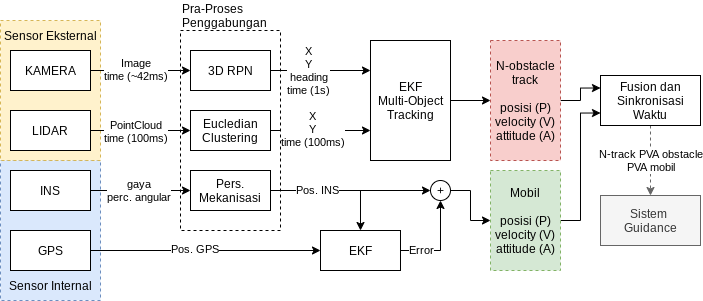
\includegraphics[width=\textwidth]{3-sistem-v7.png}
    \end{center}
\end{frame}


\begin{frame}
    \frametitle{Rencana Implementasi: Pemasangan Perangkat}
    \begin{columns}
        \begin{column}{0.3\textwidth}
            \begin{center}
                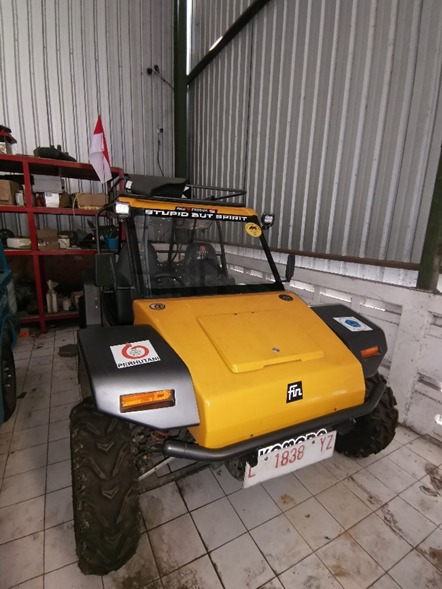
\includegraphics[width=\textwidth]{3-finn.jpeg}
            \end{center}
        \end{column}
        \begin{column}{0.65\textwidth}
            \begin{enumerate}
                \item Kamera \\
                Kamera diletakkan di sisi depan mobil, berada tepat di atas kaca depan mobil dengan arah kamera menghadap searah dengan arah gerak maju mobil.

                \item Lidar \\
                Lidar diletakkan di atap mobil agar dapat mengamati area di sekeliling mobil.

                \item INS dan GPS \\
                INS dan GPS diletakkan pada bagian bawah lantai mobil di bagian tengah mobil agar semakin dekat ke titik berat mobil untuk mengurangi bias giroskop secara keseluruhan. Antenna dari GPS diletakkan di atap mobil agar mudah mendapatkan sinyal GPS.
            \end{enumerate}
        \end{column}
    \end{columns}
\end{frame}


\begin{frame}[allowframebreaks]
    \frametitle{Rencana Implementasi: Kalibrasi Kamera. Bagian}

    Untuk mengatasi distorsi pada kamera. Perlu dilakukan kompensasi pada gambar yang ditangkap oleh kamera. Model dari distorsi kamera sebelumnya telah dibahas pada \cite{richardsz2021cv} dan tutorial dasar library OpenCV dimana distorsi radial dimodelkan sebagai

    \begin{equation}
        \left[\begin{array}{l}
        x_{d} \\
        y_{d}
        \end{array}\right]=\left(1+k_{1} r^{2}+k_{2} r^{4}+k_{3} r^{6}\right)\left[\begin{array}{l}
        x \\
        y
        \end{array}\right]
    \end{equation}

    sementara model distorsi tangensial dimodelkan sebagai

    \begin{equation}
        \left[\begin{array}{l}
        x_{d} \\
        y_{d}
        \end{array}\right]=\left[\begin{array}{l}
        x \\
        y
        \end{array}\right]+\left[\begin{array}{l}
        2 p_{1} x y+p_{2}\left(r^{2}+2 x^{2}\right) \\
        2 p_{2} x y+p_{1}\left(r^{2}+2 y^{2}\right)
        \end{array}\right]
    \end{equation}

    kita perlu mencari lima parameter distorsi $k_1, k_2, k_3, p_1,$ dan $p_2$ agar dapat menghilangkan distorsi. Selain itu, kita juga memerlukan parameter intrinsik dan ekstrinsik dari kamera seperti panjang focal lensa $f_x, f_y$ dan titik tengah optik $c_x, c_y$.

    \begin{center}
        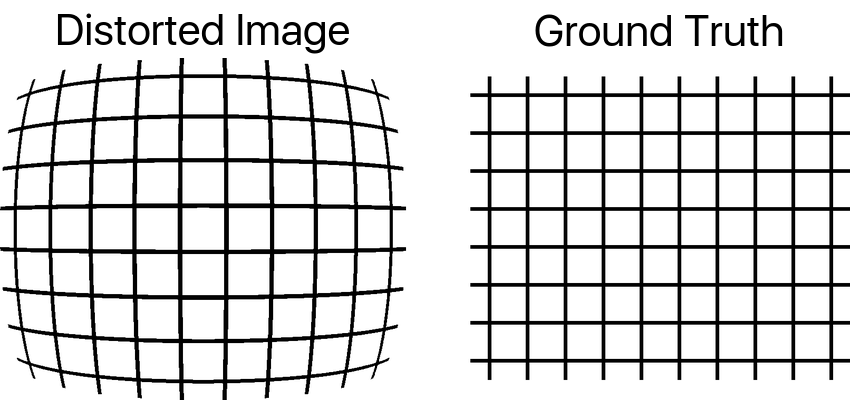
\includegraphics[width=.5\textwidth]{3-cam-distrotion.png}        
    \end{center}
\end{frame}


\begin{frame}
    \frametitle{Rencana Pengujian}
    \justifying
    Pengujian akan dilakukan untuk membuktikan hipotesa yang telah dibuat. Rencana pengujian yang akan dibuat adalah sebagai berikut:
    \begin{itemize}
        \item Pengujian hasil deteksi posisi halangan
        \item Pengujian posisi mobil
        \item Pengujian fusion Internal dan Eksternal
    \end{itemize}
\end{frame}


\begin{frame}
    \frametitle{Pengujian hasil deteksi posisi halangan}
    \justifying
    Pengujian ini dilakukan untuk menguji hasil sensor fusion kamera dengan lidar yang dihasilkan oleh EKF Multi-Object Tracking. Pengujian hasil deteksi posisi halangan ini akan dilakukan dengan beberapa variasi jarak dan jumlah halangan. Pengujian ini akan dilakukan dengan menggunakan data yang telah diperoleh dari sensor fusion kamera dengan lidar, dibandingkan dengan data pengukuran manual.
\end{frame}


\begin{frame}
    \frametitle{Pengujian posisi mobil}
    \justifying
    Pengujian ini dilakukan untuk menguji hasil sensor fusion dari GPS dan INS yang dihasilkan oleh EKF. Pengujian hasil deteksi posisi mobil otonom ini akan dilakukan dengan beberapa variasi lintasan, yakni:
    \begin{enumerate}
        \item lintasan lurus
        \item lintasan memutar
        \item lintasan berliku
    \end{enumerate}
\end{frame}


\begin{frame}
    \frametitle{Pengujian metode tracking}
    \justifying
    Pengujian ini dilakukan untuk menguji hasil tracking yang dihasilkan oleh metode fusion tahap akhir pada:
    \begin{enumerate}
        \item Satu objek statik
        \item Dua objek statik
        \item skenario halangan 1 mendahului halangan 2.
        \item skenario halangan 1 berpapasan dengan halangan 2.
    \end{enumerate}
\end{frame}